\documentclass{article}

\usepackage{amsmath}
\usepackage{amssymb}
\usepackage{array}
\usepackage{booktabs}
\usepackage{graphicx}
\usepackage[margin=1in]{geometry}
\usepackage[hidelinks]{hyperref}
\usepackage{xurl}

\graphicspath{{figures/}}
\hypersetup{linktoc=all}

\newcommand{\ee}{\ensuremath{e^+e^-}}
\newcommand{\pT}{\ensuremath{p_{\mathrm{T}}}}
\newcommand{\vn}[2]{\ensuremath{v_{#1}\{#2\}}}
\newcommand{\cn}[2]{\ensuremath{c_{#1}\{#2\}}}
\newcommand{\avg}[1]{\ensuremath{\left\langle #1 \right\rangle}}

\title{Analysis note: charged-particle multi-particle cumulants in ALEPH hadronic \(\ee\) collisions at the \(Z\) pole}
\author{Yen-Jie Lee}
\date{June 16, 2026}

\begin{document}

\maketitle

\begin{abstract}
This note documents a first charged-particle multi-particle cumulant analysis
of archived ALEPH hadronic \(e^+e^-\) collisions at \(\sqrt{s}\simeq91.2\) GeV.
The analysis follows the public Electron-Positron Alliance note style: the
main body defines the observable, data setup, event and track selections,
cumulant calculation, statistical uncertainty treatment, and the current
preliminary results. The reported observables are \(\vn{2}{2}\),
\(\vn{2}{4}\), \(\vn{2}{6}\), and \(\vn{2}{8}\) as functions of selected
charged-particle multiplicity, evaluated with respect to both the laboratory
beam axis and the event thrust axis. The cumulant implementation uses exact
ordered, distinct-particle correlations through eighth order and propagates
statistical uncertainties with delete-one-chunk jackknife resampling over
sixteen event chunks. The present result is a detector-level charged-particle
study; detector-response, acceptance, and model-dependent systematic
uncertainties are not yet included. A matched 1994 reconstructed-MC comparison
is included as a baseline closure-style check of the beam-axis and thrust-axis
trends.
\end{abstract}

\noindent\textbf{Keywords:} ALEPH, archived \(e^+e^-\) data, charged-particle
cumulants, flow harmonics, Q-cumulants

\tableofcontents
\clearpage

\section{Introduction}

Long-range azimuthal correlations and multi-particle cumulants are central
tools for separating collective and non-collective correlation structures in
high-energy collisions. In hadronic and nuclear collisions, the hierarchy of
\(\vn{n}{2}\), \(\vn{n}{4}\), \(\vn{n}{6}\), and \(\vn{n}{8}\) provides a
compact way to test whether the measured azimuthal anisotropy is dominated by a
common event-level geometry or by few-particle correlations. The same
techniques can be applied to archived \(e^+e^-\) data, where the absence of
beam remnants and a well-defined color-singlet initial state provide a clean
reference for jet fragmentation, parton-shower, and hadronization effects.

The starting point for this analysis is the ALEPH StudyMult charged-particle
workflow and the previous ALEPH two-particle-correlation analysis of archived
LEP data~\cite{Badea:2019vey}. The present note extends that infrastructure
from two-particle Fourier coefficients to exact multi-particle cumulants
through eight particles. The implementation follows the Q-cumulant formalism
of Refs.~\cite{Bilandzic:2010jr,Bilandzic:2013kga} and the cumulant
combinations used in small-system flow measurements, including the CMS
high-multiplicity pp reference analysis~\cite{CMS:2016fnw}.

This document intentionally follows the compact public-note format used in
recent Electron-Positron Alliance analysis notes. The main body contains the
observable definition, active data setup, analysis method, validation, and
preliminary results, while detailed corrections and systematic variations are
identified as future work rather than folded into the present detector-level
result.

\section{Observable Definition}
\label{sec:observable}

For each selected event, charged particles are represented by their azimuthal
angles \(\phi_i\) in a chosen coordinate system. The present study uses two
coordinate definitions:
\begin{itemize}
  \item beam axis: \(\phi_i\) is the laboratory azimuth around the ALEPH beam
  axis;
  \item thrust axis: the event is rotated into a frame defined by the event
  thrust axis, and \(\phi_i\) is the azimuth around that axis.
\end{itemize}

The harmonic used in this note is \(n=2\). For an event with multiplicity
\(M\), the ordered distinct-particle \(2k\)-particle correlation is
\begin{equation}
  \avg{2k}_{n}
  =
  \frac{1}{M(M-1)\cdots(M-2k+1)}
  \sum_{\substack{i_1,\ldots,i_{2k}\\ \mathrm{all~distinct}}}
  \exp\left[
    in\left(\phi_{i_1}+\cdots+\phi_{i_k}
    -\phi_{i_{k+1}}-\cdots-\phi_{i_{2k}}\right)
  \right].
  \label{eq:ordered-correlation}
\end{equation}
The event-ensemble averages of these quantities are accumulated with their
natural ordered-tuple weights. The cumulants are then
\begin{align}
  \cn{2}{2} &= \avg{2}, \\
  \cn{2}{4} &= \avg{4} - 2\avg{2}^2, \\
  \cn{2}{6} &= \avg{6} - 9\avg{4}\avg{2} + 12\avg{2}^3, \\
  \cn{2}{8} &= \avg{8} - 16\avg{6}\avg{2} - 18\avg{4}^2
              + 144\avg{4}\avg{2}^2 - 144\avg{2}^4 .
  \label{eq:cumulants}
\end{align}
The corresponding flow-like coefficients are defined as
\begin{align}
  \vn{2}{2} &= \sqrt{\cn{2}{2}}, \\
  \vn{2}{4} &= \left[-\cn{2}{4}\right]^{1/4}, \\
  \vn{2}{6} &= \left[\cn{2}{6}/4\right]^{1/6}, \\
  \vn{2}{8} &= \left[-\cn{2}{8}/33\right]^{1/8}.
  \label{eq:vndefs}
\end{align}
If the required cumulant sign is not physical for a given bin, the
corresponding \(\vn{2}{m}\) point is suppressed in the plotted result and is
stored as zero in the exported CSV table.

\section{Data Setup and Selections}
\label{sec:data}

The current production uses the local StudyMult-format ALEPH file
\begin{center}
\path{/data/yjlee/StudyMult/DataFiles/ROOTfiles/cleaned_ALEPH_Data-all.aleph.root}.
\end{center}
This file contains \(59{,}874\) selected hadronic events in the tree
\texttt{t}. The input format is the StudyMult fixed-array layout with
\texttt{nParticle}, \texttt{px}, \texttt{py}, \texttt{pz}, and
\texttt{pwflag} branches.

Charged particles are selected using the StudyMult charged-particle convention
\begin{equation}
  \texttt{pwflag}\in\{0,1,2\},
\end{equation}
with \(\pT>0.4\) GeV for both the beam-axis and thrust-axis cumulants. The
event thrust axis is computed from reconstructed particle momenta, following
the local ALEPH StudyMult convention used by the prototype analyses. The
charged-particle multiplicity bins used in this note are
\[
  [0,10), [10,15), [15,20), [20,25), [25,30), [30,35), [35,40), [40,\infty).
\]
The corresponding event counts are shown in Table~\ref{tab:event-counts}.

\begin{table}[htbp]
\centering
\caption{Selected event counts in the multiplicity bins used for the current
detector-level cumulant analysis.}
\label{tab:event-counts}
\begin{tabular}{lc}
\toprule
Multiplicity bin & Events \\
\midrule
\([0,10)\) & 7483 \\
\([10,15)\) & 17665 \\
\([15,20)\) & 16856 \\
\([20,25)\) & 9452 \\
\([25,30)\) & 4753 \\
\([30,35)\) & 2287 \\
\([35,40)\) & 955 \\
\([40,\infty)\) & 423 \\
\bottomrule
\end{tabular}
\end{table}

\section{Cumulant Implementation}
\label{sec:method}

The analysis code computes the ordered correlations in
Eq.~\eqref{eq:ordered-correlation} using an exact elementary-symmetric
polynomial recursion over the event-level phase factors
\(\exp(in\phi_i)\). This avoids self-correlations by construction and uses the
same ordered-particle denominator as the Q-cumulant definition. The recursion
is applied for \(2\), \(4\), \(6\), and \(8\) particles in each multiplicity bin
and for both axis definitions.

The implementation was checked in two ways. First, the code contains a
\texttt{--SelfTest 1} mode that compares the production correlator against
brute-force ordered distinct-particle sums for low-multiplicity toy events.
Second, the cumulant combinations and \(\vn{2}{m}\) normalizations were compared
against the published Q-cumulant formulae in
Refs.~\cite{Bilandzic:2010jr,Bilandzic:2013kga,CMS:2016fnw}. The signs and
normalization factors in the cumulant and \(\vn{2}{m}\) definitions above match
those references.

\section{Statistical Uncertainties}
\label{sec:statistics}

The production job was split into sixteen contiguous event chunks. Each chunk
stores independent numerator and denominator sums for every correlator and
multiplicity bin. The summary step first merges all chunks to obtain the
central value and then recomputes the full nonlinear cumulant chain after
removing one chunk at a time. The quoted statistical uncertainty is the
delete-one-chunk jackknife estimate
\begin{equation}
  \sigma_{\mathrm{JK}} =
  \sqrt{\frac{N_{\mathrm{chunk}}-1}{N_{\mathrm{chunk}}}
  \sum_{j=1}^{N_{\mathrm{chunk}}}
  \left(x_{(j)}-\bar{x}\right)^2},
\end{equation}
where \(x_{(j)}\) is the result with chunk \(j\) removed. This propagates the
nonlinear transformations from raw correlations to cumulants and then to
\(\vn{2}{m}\). The procedure assumes the chunks are statistically independent;
if the input file ordering tracks detector running conditions, the jackknife
may also contain a small run-block component.

\section{Preliminary Results}
\label{sec:results}

Figures~\ref{fig:v2-beam} and~\ref{fig:v2-thrust} show the current
detector-level \(\vn{2}{2}\), \(\vn{2}{4}\), \(\vn{2}{6}\), and \(\vn{2}{8}\)
results versus charged-particle multiplicity. In both coordinate systems the
two-particle value is larger than the higher-order values, as expected when
few-particle and jet-like correlations contribute. The higher-order beam-axis
points remain numerically stable through most bins, while some high-order
thrust-axis and high-multiplicity points become sign-unstable or carry large
jackknife uncertainties because the event counts and ordered eight-particle
statistics are limited in those bins.

\begin{figure}[htbp]
  \centering
  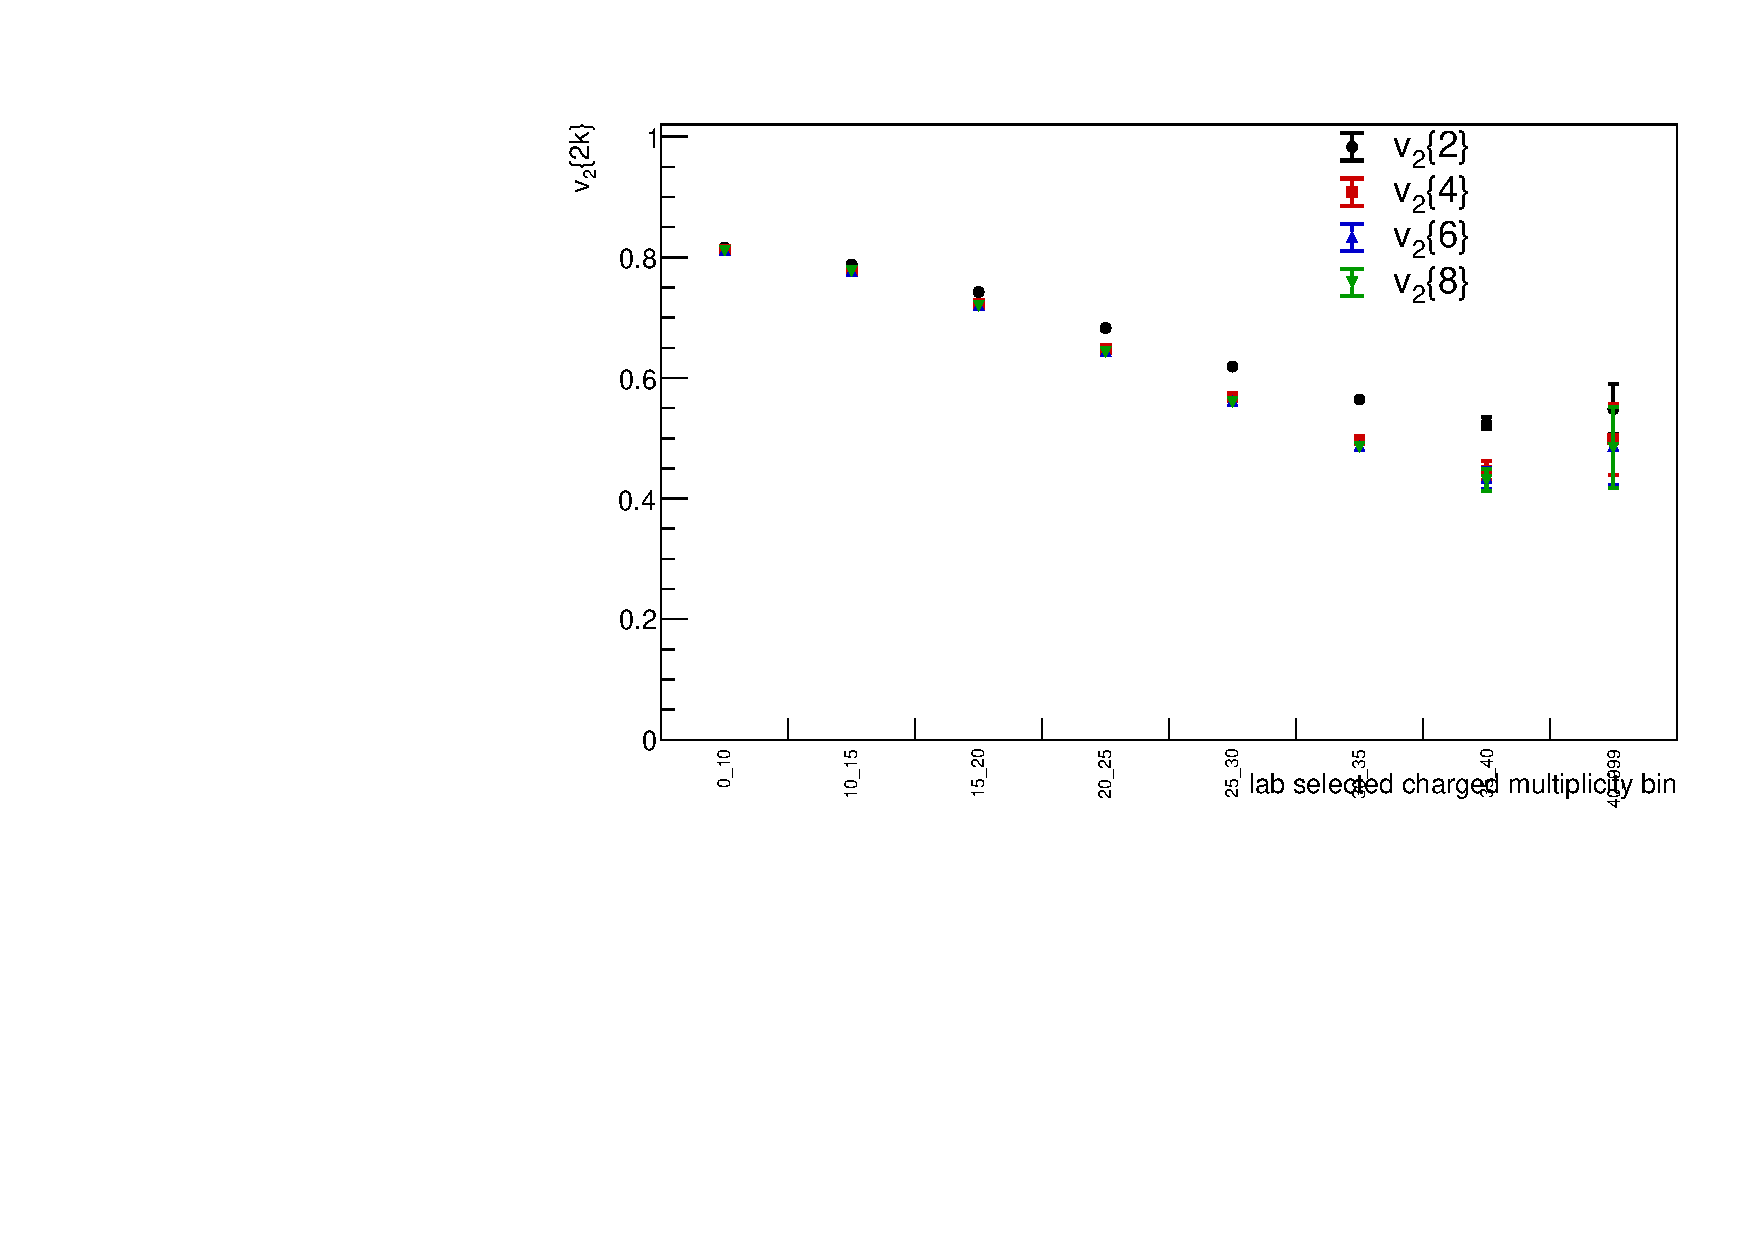
\includegraphics[width=0.92\textwidth]{v2_multiplicity_beam.pdf}
  \caption{Detector-level charged-particle \(\vn{2}{2}\), \(\vn{2}{4}\),
  \(\vn{2}{6}\), and \(\vn{2}{8}\) as functions of selected charged-particle
  multiplicity using the laboratory beam-axis azimuth. Error bars are
  delete-one-chunk jackknife statistical uncertainties from sixteen event
  chunks. Missing high-order points indicate cumulant signs that do not give a
  real-valued \(\vn{2}{m}\) in the current sample.}
  \label{fig:v2-beam}
\end{figure}

\begin{figure}[htbp]
  \centering
  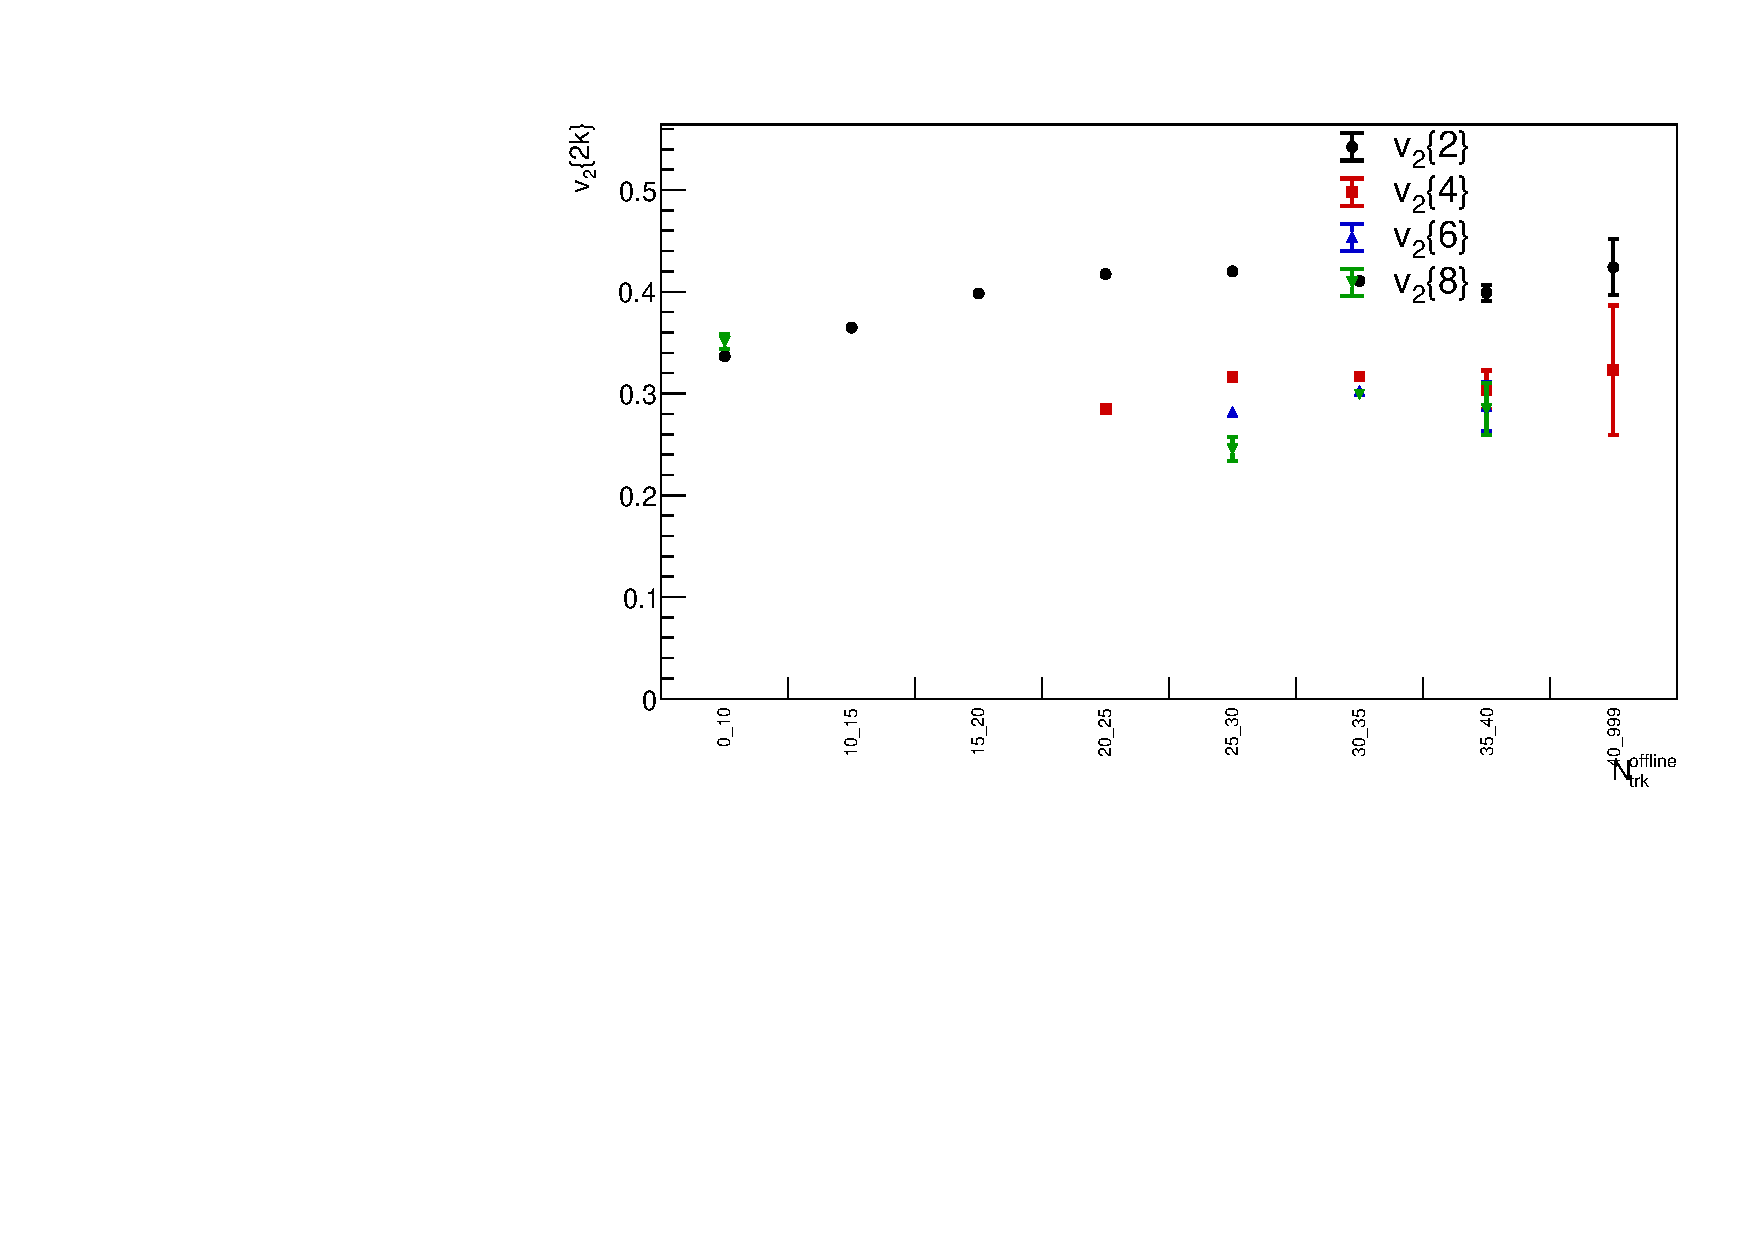
\includegraphics[width=0.92\textwidth]{v2_multiplicity_thrust.pdf}
  \caption{Detector-level charged-particle \(\vn{2}{2}\), \(\vn{2}{4}\),
  \(\vn{2}{6}\), and \(\vn{2}{8}\) as functions of selected charged-particle
  multiplicity using azimuth around the event thrust axis. Error bars are
  delete-one-chunk jackknife statistical uncertainties from sixteen event
  chunks.}
  \label{fig:v2-thrust}
\end{figure}

\begin{table}[htbp]
\centering
\small
\caption{Numerical beam-axis \(\vn{2}{m}\) values. Uncertainties are
jackknife statistical uncertainties. Entries shown as ``--'' are sign-invalid
or unavailable in the current sample.}
\label{tab:beam-results}
\begin{tabular}{lcccc}
\toprule
Multiplicity & \(\vn{2}{2}\) & \(\vn{2}{4}\) & \(\vn{2}{6}\) & \(\vn{2}{8}\) \\
\midrule
\([0,10)\) & \(0.7277\pm0.0024\) & \(0.7047\pm0.0032\) & \(0.7031\pm0.0034\) & \(0.7029\pm0.0034\) \\
\([10,15)\) & \(0.7182\pm0.0027\) & \(0.6802\pm0.0040\) & \(0.6757\pm0.0041\) & \(0.6748\pm0.0042\) \\
\([15,20)\) & \(0.7109\pm0.0023\) & \(0.6705\pm0.0038\) & \(0.6654\pm0.0041\) & \(0.6645\pm0.0042\) \\
\([20,25)\) & \(0.6720\pm0.0029\) & \(0.6210\pm0.0045\) & \(0.6140\pm0.0049\) & \(0.6125\pm0.0050\) \\
\([25,30)\) & \(0.6114\pm0.0044\) & \(0.5372\pm0.0070\) & \(0.5251\pm0.0077\) & \(0.5222\pm0.0079\) \\
\([30,35)\) & \(0.5332\pm0.0046\) & \(0.4265\pm0.0080\) & \(0.3982\pm0.0120\) & \(0.3847\pm0.0169\) \\
\([35,40)\) & \(0.4823\pm0.0079\) & \(0.3506\pm0.0184\) & \(0.2981\pm0.0481\) & -- \\
\([40,\infty)\) & \(0.4469\pm0.0093\) & \(0.3018\pm0.0297\) & -- & -- \\
\bottomrule
\end{tabular}
\end{table}

\begin{table}[htbp]
\centering
\small
\caption{Numerical thrust-axis \(\vn{2}{m}\) values. Uncertainties are
jackknife statistical uncertainties. Entries shown as ``--'' are sign-invalid
or unavailable in the current sample.}
\label{tab:thrust-results}
\begin{tabular}{lcccc}
\toprule
Multiplicity & \(\vn{2}{2}\) & \(\vn{2}{4}\) & \(\vn{2}{6}\) & \(\vn{2}{8}\) \\
\midrule
\([0,10)\) & \(0.6655\pm0.0045\) & \(0.6034\pm0.0068\) & \(0.5958\pm0.0070\) & \(0.5938\pm0.0072\) \\
\([10,15)\) & \(0.6627\pm0.0039\) & \(0.5748\pm0.0056\) & \(0.5515\pm0.0065\) & \(0.5431\pm0.0071\) \\
\([15,20)\) & \(0.6300\pm0.0051\) & \(0.5294\pm0.0068\) & \(0.4962\pm0.0078\) & \(0.4791\pm0.0090\) \\
\([20,25)\) & \(0.5582\pm0.0046\) & \(0.4341\pm0.0063\) & \(0.3787\pm0.0114\) & \(0.2828\pm0.4437\) \\
\([25,30)\) & \(0.4810\pm0.0025\) & \(0.3535\pm0.0066\) & \(0.2963\pm0.0180\) & -- \\
\([30,35)\) & \(0.4488\pm0.0050\) & \(0.3359\pm0.0094\) & \(0.3011\pm0.0212\) & \(0.2802\pm0.0490\) \\
\([35,40)\) & \(0.4231\pm0.0071\) & \(0.3294\pm0.0118\) & \(0.3125\pm0.0166\) & \(0.3094\pm0.0200\) \\
\([40,\infty)\) & \(0.4151\pm0.0101\) & \(0.3084\pm0.0189\) & \(0.2475\pm0.0754\) & -- \\
\bottomrule
\end{tabular}
\end{table}


\subsection{Matched 1994 reconstructed-MC comparison}
\label{subsec:mc-comparison}

A separate MC production was run on the matched LEP1 1994 reconstructed-MC
sample
\begin{center}
\path{/data/yjlee/ALEPH_Agentic_Event_Shape_Analysis/DataProcessing/temp/alephMCRecoAfterCutPaths_1994_thrust_pt04_t.root}.
\end{center}
For a like-for-like comparison, the corresponding 1994 data sample
\begin{center}
\path{/data/yjlee/ALEPH_Agentic_Event_Shape_Analysis/DataProcessing/temp/LEP1Data1994_recons_aftercut-MERGED_thrust_pt04_t.root}
\end{center}
was processed with the same cumulant settings, multiplicity bins, and
sixteen-chunk jackknife procedure. The processed input contains 771,597 MC
entries and 1,365,440 data entries. These samples are separate from the
all-StudyMult data-only production shown above, and are used only for the
reconstructed-level data/MC comparison in this subsection.

Figures~\ref{fig:v2-mc-beam} and~\ref{fig:v2-mc-thrust} show the standalone MC
result for the beam and thrust axes. The beam-axis MC follows the same broad
multiplicity dependence as the data-only result: the cumulant hierarchy is tight
at low multiplicity and decreases with increasing multiplicity. In the thrust
axis, the two-particle coefficient rises from low to intermediate multiplicity,
while several low-multiplicity higher-order coefficients are sign-invalid and
therefore not plotted.

\begin{figure}[htbp]
  \centering
  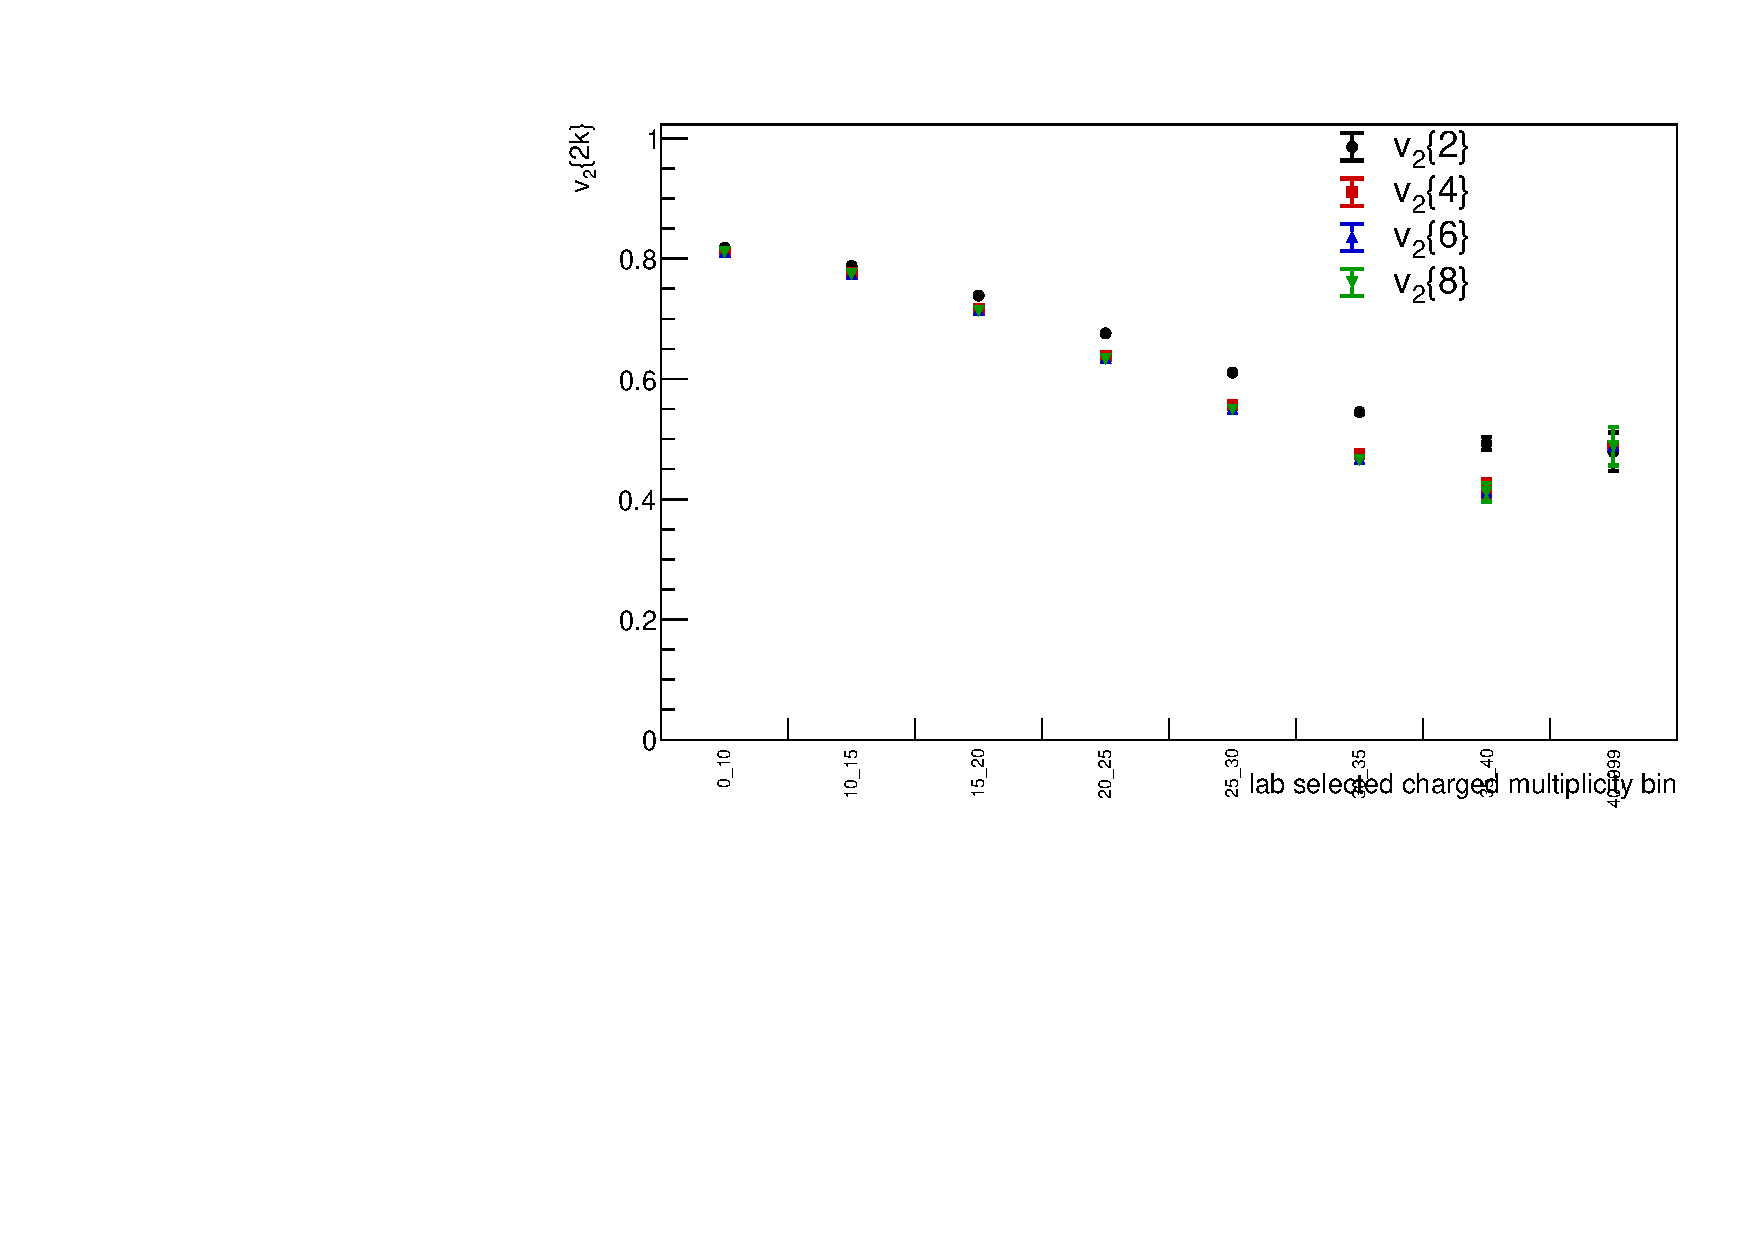
\includegraphics[width=0.92\textwidth]{v2_multiplicity_mc_beam.pdf}
  \caption{Matched LEP1 1994 reconstructed-MC \(\vn{2}{2}\), \(\vn{2}{4}\),
  \(\vn{2}{6}\), and \(\vn{2}{8}\) versus selected charged-particle
  multiplicity using the laboratory beam-axis azimuth.}
  \label{fig:v2-mc-beam}
\end{figure}

\begin{figure}[htbp]
  \centering
  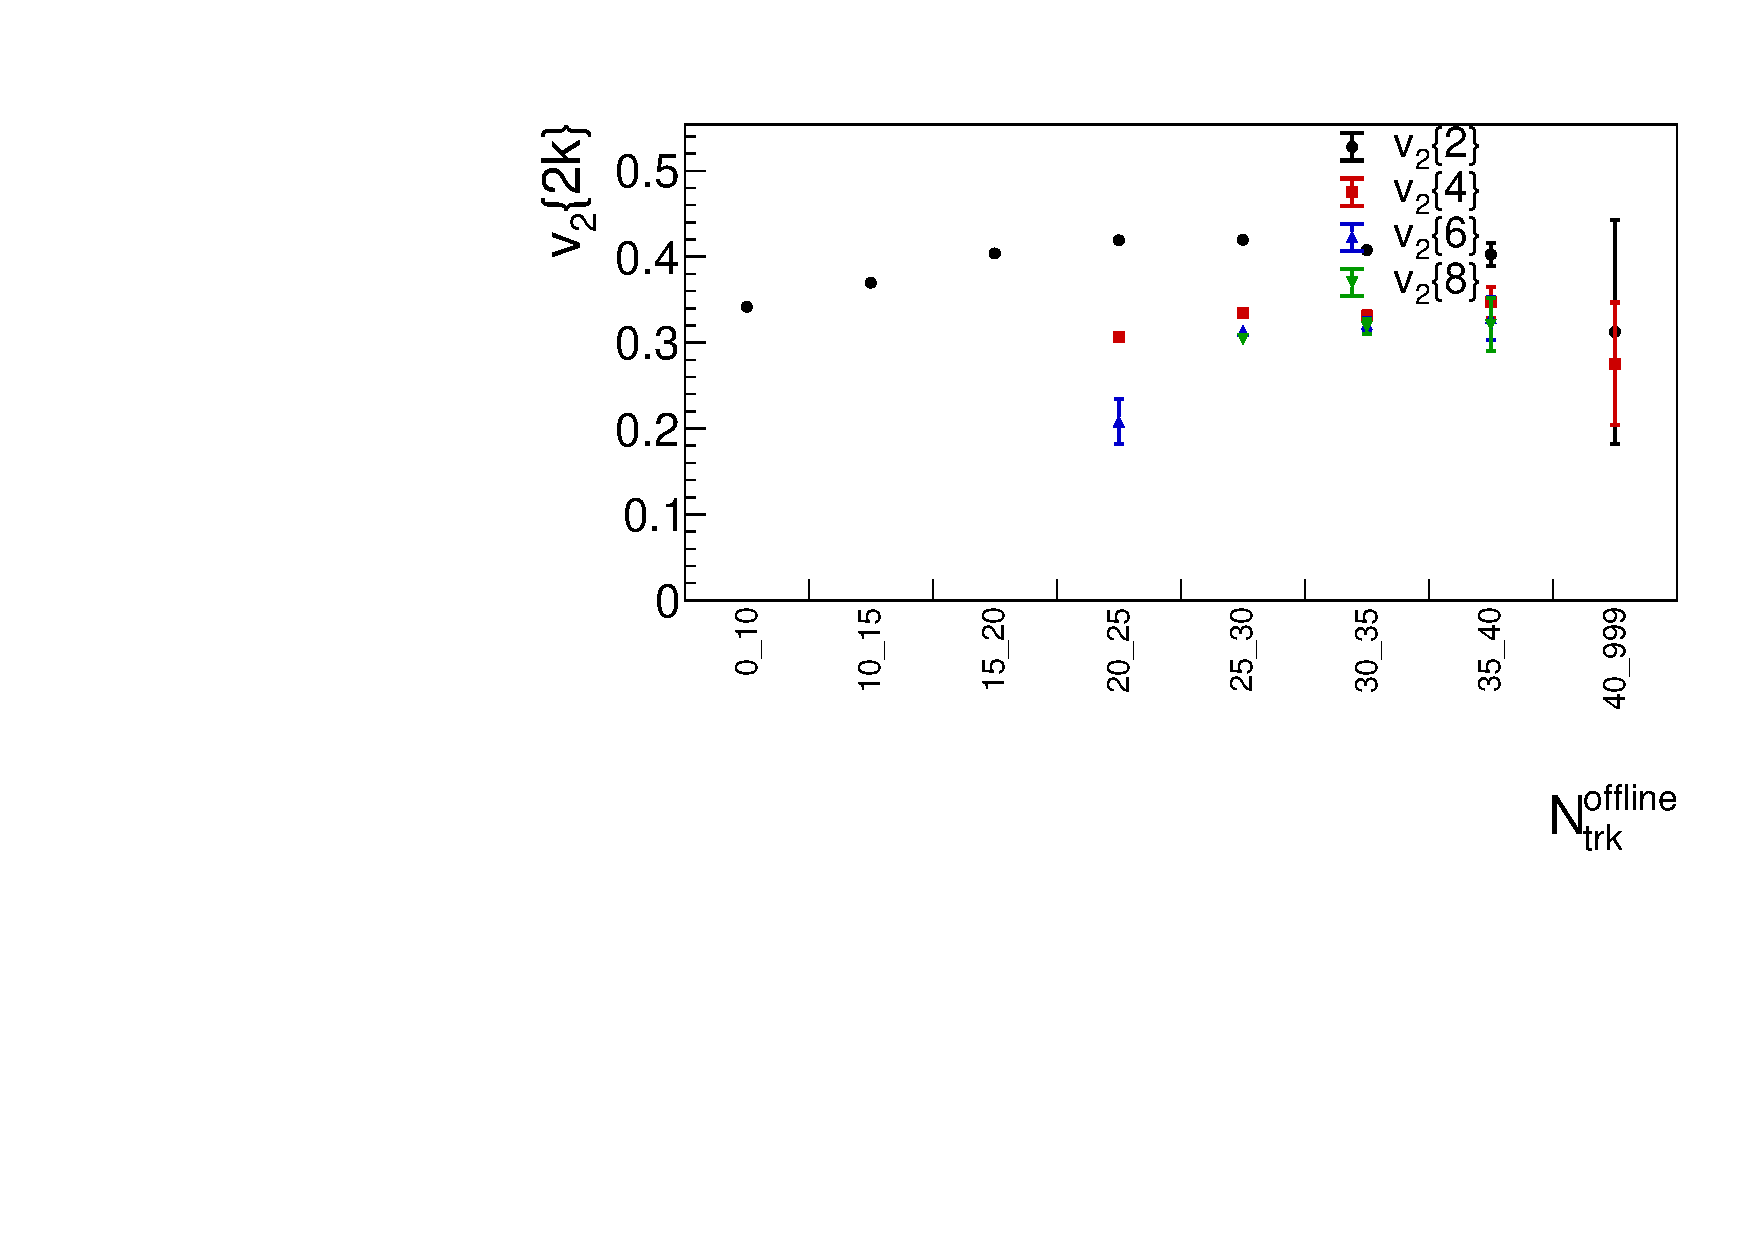
\includegraphics[width=0.92\textwidth]{v2_multiplicity_mc_thrust.pdf}
  \caption{Matched LEP1 1994 reconstructed-MC \(\vn{2}{2}\), \(\vn{2}{4}\),
  \(\vn{2}{6}\), and \(\vn{2}{8}\) versus selected charged-particle
  multiplicity using azimuth around the event thrust axis.}
  \label{fig:v2-mc-thrust}
\end{figure}

Figures~\ref{fig:v2-data-mc-beam} and~\ref{fig:v2-data-mc-thrust} compare the
matched 1994 data and reconstructed MC directly. For the beam axis, the data/MC
agreement is at the percent level over most of the populated multiplicity range;
the largest deviations appear in the highest-multiplicity bin, where the
statistical uncertainty is also largest. For the thrust axis, \(\vn{2}{2}\) is
well reproduced through intermediate multiplicity. The higher-order thrust-axis
coefficients are more sensitive to cumulant sign changes and limited statistics,
so missing points indicate bins where either data or MC did not yield a real
value under the standard cumulant sign convention.

\begin{figure}[htbp]
  \centering
  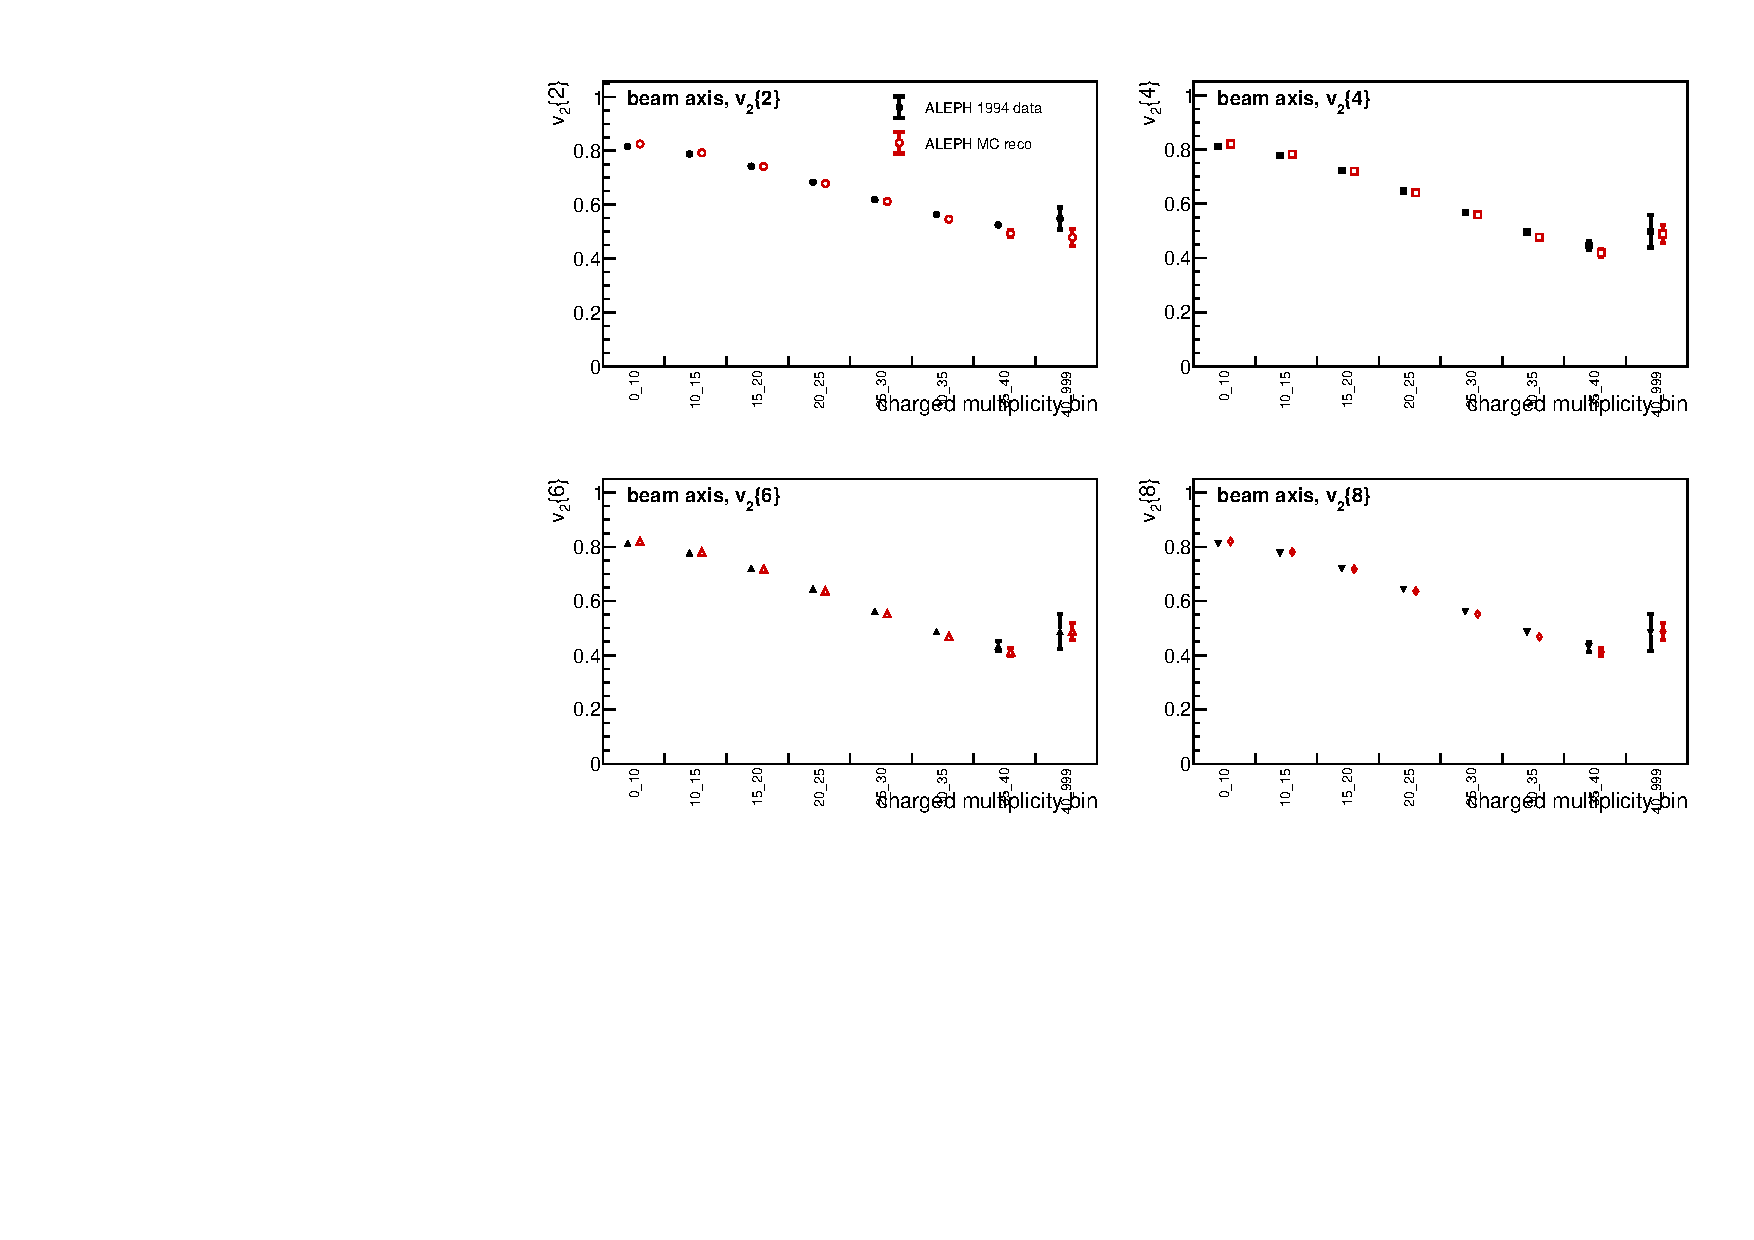
\includegraphics[width=0.98\textwidth]{v2_data_mc_compare_beam.pdf}
  \caption{Beam-axis comparison of matched LEP1 1994 data and reconstructed MC.
  Each panel shows one cumulant order, with data and MC offset slightly in the
  charged-multiplicity bin for readability.}
  \label{fig:v2-data-mc-beam}
\end{figure}

\begin{figure}[htbp]
  \centering
  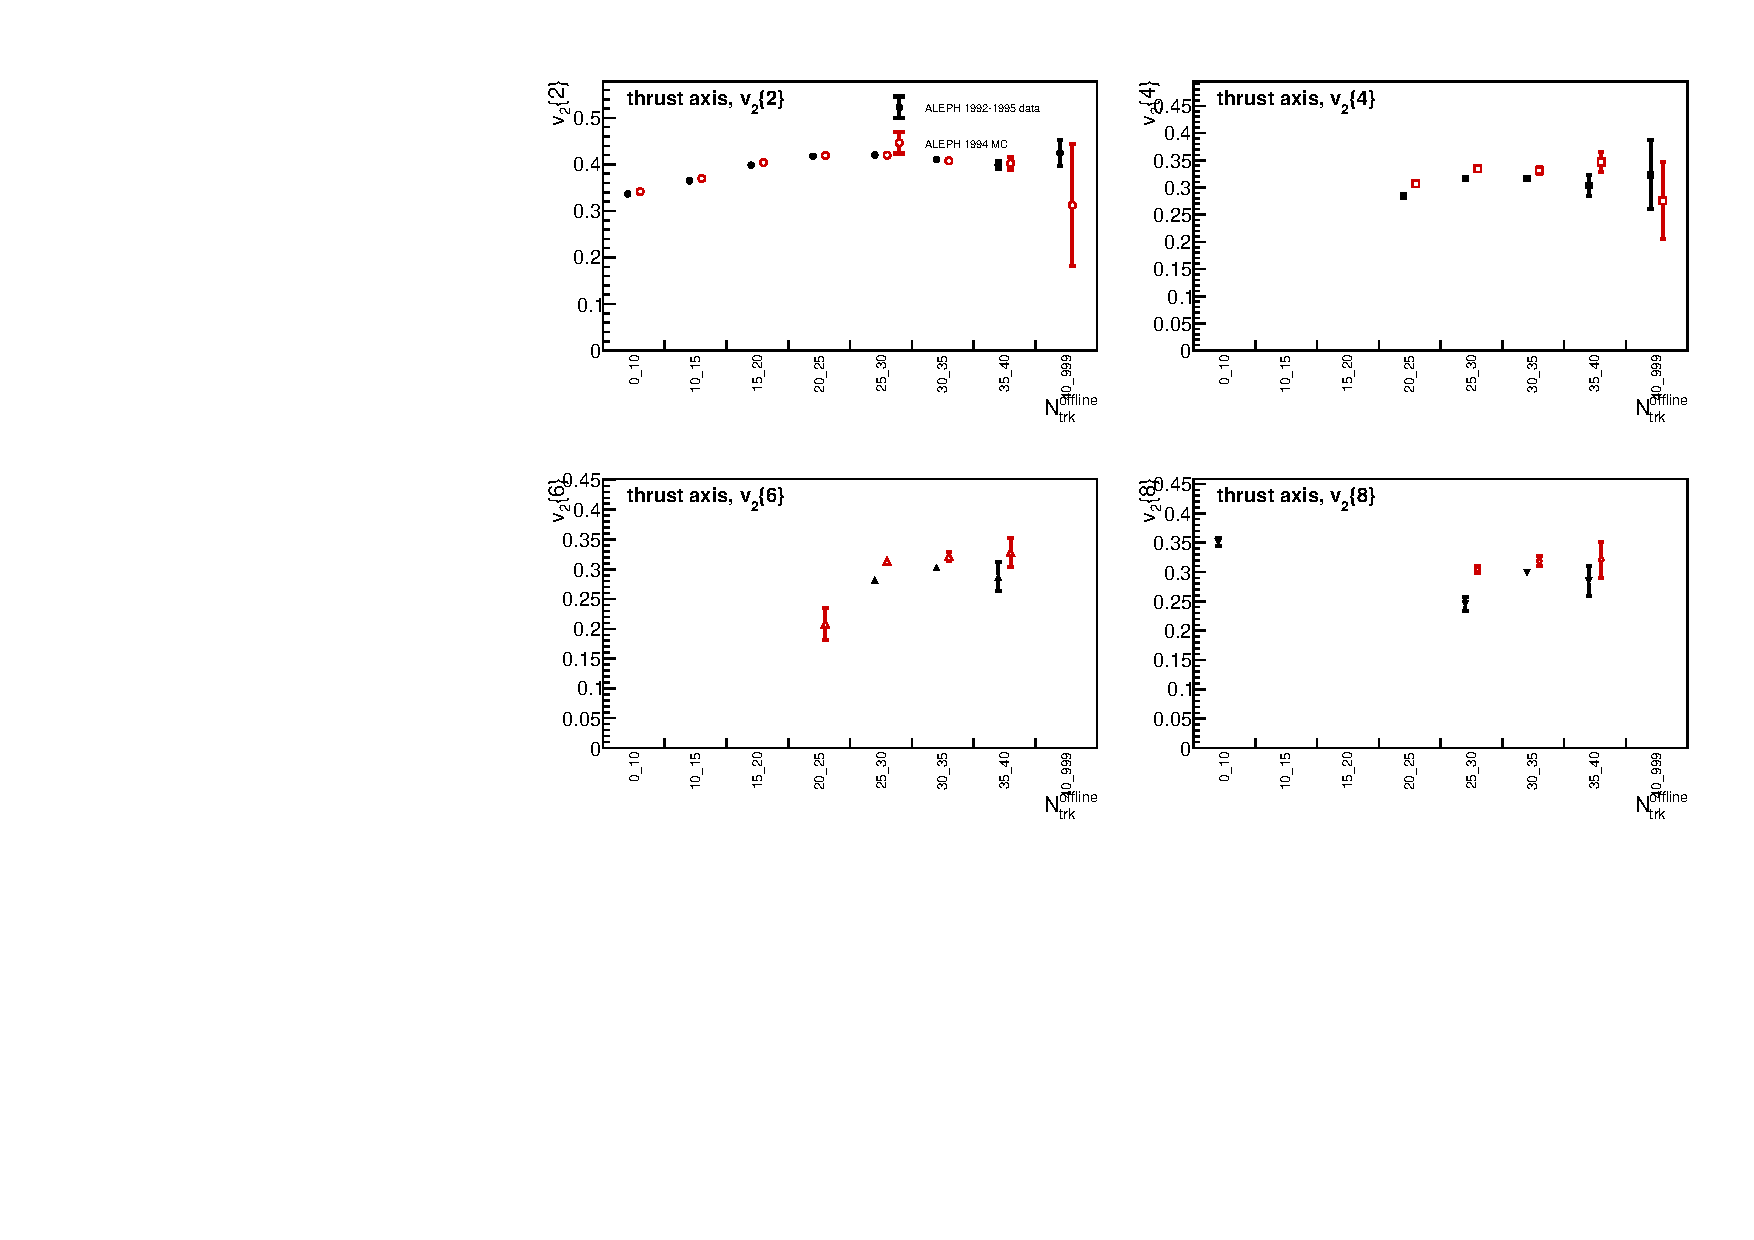
\includegraphics[width=0.98\textwidth]{v2_data_mc_compare_thrust.pdf}
  \caption{Thrust-axis comparison of matched LEP1 1994 data and reconstructed
  MC. Missing high-order points correspond to sign-invalid cumulants or bins
  without a valid real-valued \(\vn{2}{m}\).}
  \label{fig:v2-data-mc-thrust}
\end{figure}

\section{Current Limitations}
\label{sec:limitations}

The present note should be read as a detector-level analysis milestone, not as a
final corrected physics result. The main limitations are:
\begin{itemize}
  \item no detector-response or acceptance correction is applied to the
  cumulants;
  \item the current reconstructed-MC comparison is a baseline check, not a
  detector-response correction or generator systematic uncertainty;
  \item no variation of the track \(\pT\) threshold, charged-particle
  definition, thrust-axis construction, or event-selection definition is
  included yet;
  \item high-order cumulants in the highest-multiplicity bins are statistically
  fragile and can become sign-invalid.
\end{itemize}
These items define the next analysis steps before the result can be interpreted
as a corrected ALEPH measurement.

\section{Summary}
\label{sec:summary}

A first ALEPH charged-particle cumulant workflow has been built from the local
StudyMult code base and validated against exact brute-force ordered-particle
sums. The current production processes \(59{,}874\) StudyMult events and
extracts \(\vn{2}{2}\), \(\vn{2}{4}\), \(\vn{2}{6}\), and \(\vn{2}{8}\) versus
charged-particle multiplicity for both the beam-axis and thrust-axis azimuthal
definitions. Statistical uncertainties are propagated through the nonlinear
cumulant definitions with a sixteen-chunk jackknife. The beam-axis and
thrust-axis figures included in this note provide the current detector-level
baseline for subsequent correction and systematic-uncertainty studies.

\bibliographystyle{unsrt}
\bibliography{references}

\end{document}
